\chapter{Experimental Results}

%Replace \lipsum with text.
% You may have as many sections as you please. This is just for reference.

\section{Transfer of Data from RTDS to server}
\begin{figure}
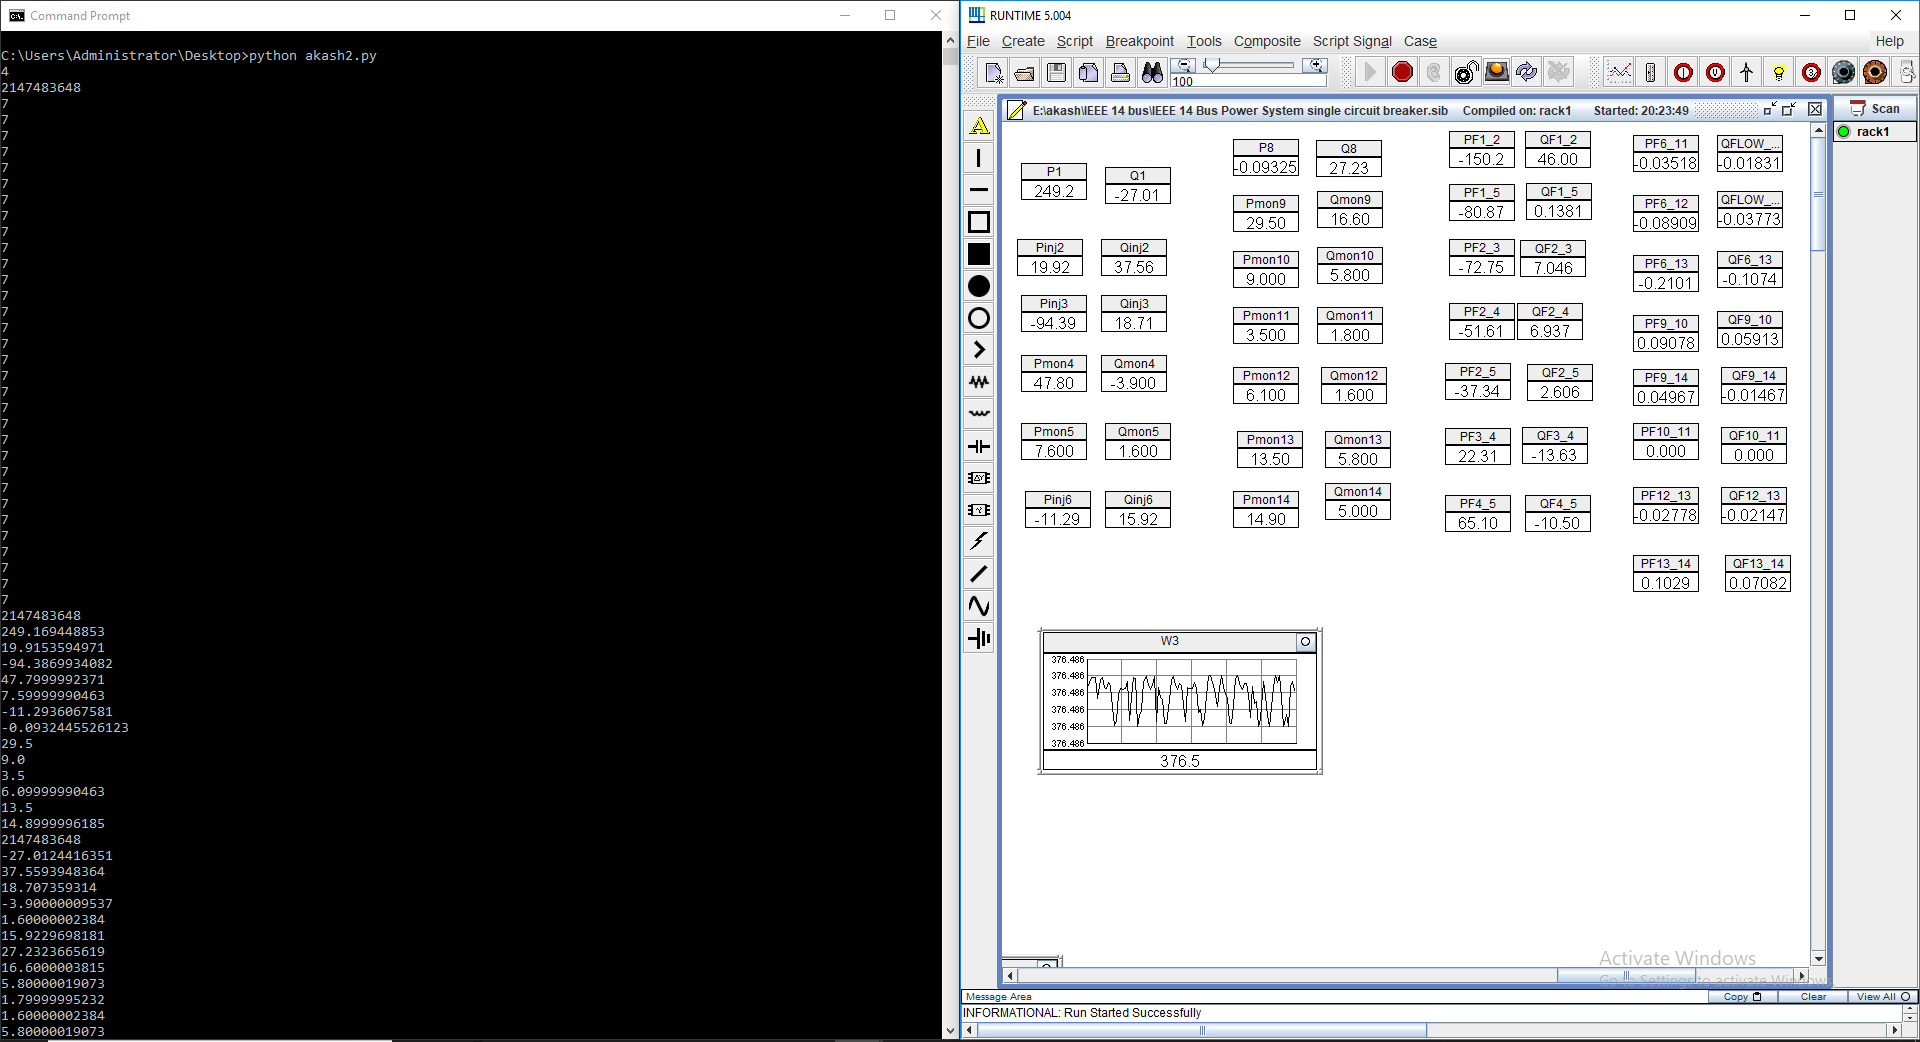
\includegraphics[width=\textwidth]{Figures/response_dt_cb.png}
\caption{Transfer of real and reactive power injections and flows from RTDS (right) to server (left), Observing circuit breaker status}
\label{fig:data_transfer_cb_status}
\end{figure}

\begin{figure}
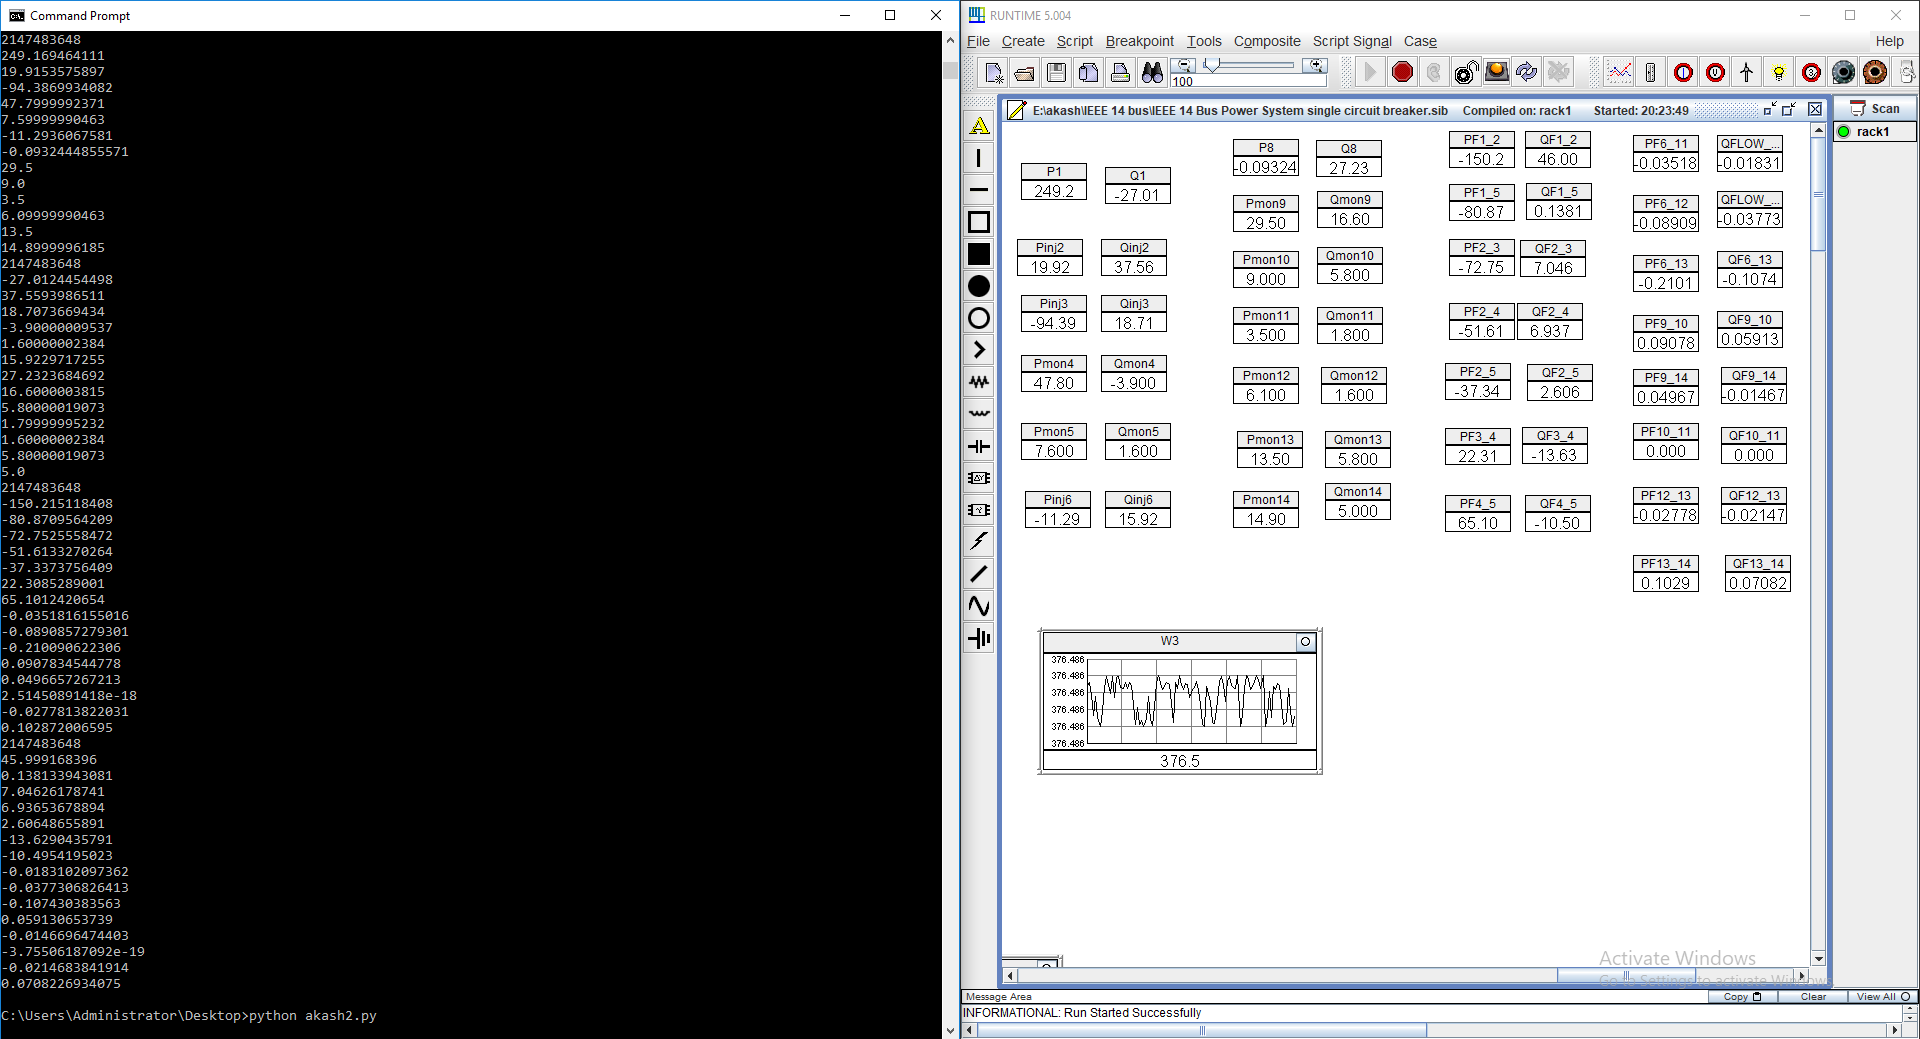
\includegraphics[width=\textwidth]{result_dt2.png}
\caption{Transfer of real and reactive power injections and flows from RTDS (right) to server (left)}
\label{fig:data_transfer}
\end{figure}

In Figure ~\ref{fig:data_transfer}, we observe real time data transfer from RTDS via GTNET-SKT to our server, which we built using a python script running on the Desktop. Here the measurements come in the order described in chapter 3 (Real injection then reactive . The value 4294967295 ($2^{32}-1$) is the status number for the set of measurements. All bits are 1, signifying all measurements are available. In Figure ~\ref{fig:data_transfer_cb_status}, we observe the availability status of all circuit breakers in the system. The first number is the case\_number, and 4 represents 14 bus system. Circuit breakers status number is also 4294967295, signifying all circuit breakers are available. Circuit breaker measurement of 7 represents all 3 phases are ON (3 bits are 1).\\
The graph is the frequency response curve of the system, in rad/s. The system operates at $376.5/2 \pi=60Hz$ with very little fluctuation.\\

This shows that we have been able to extract all the available measurements, and identify which measurement belongs to which variable, without using many extra measurement variables.

\section{Observability Analysis and State Estimation}
After collecting data, we perform observability analysis. If the system is found to be observable, we perform state estimation.
Here, for the above example, the system performs state estimation since all measurements are available. In fact, since all the measurements are available, and are exact measurements, the results obtained from state estimation are very close to the ones obtained from load flow solutions (See values at \cite{uwash_cdf}).

\begin{figure}
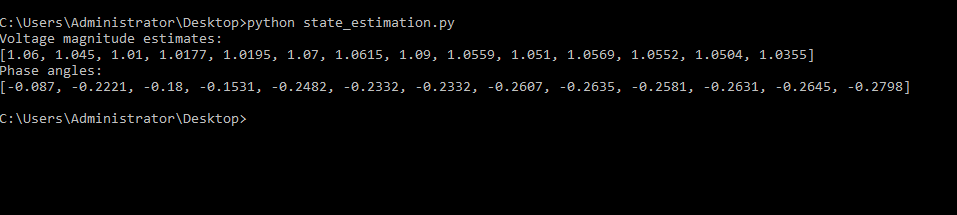
\includegraphics[width=\textwidth]{Figures/state_estimate.png}
\caption{Values of Bus voltages and angles for IEEE 14 Bus system}
\label{fig:se}
\end{figure}

To create an unobservable system, we modify the availability of line flow and bus injection datas, and try finding out the state estimates. We removed the real and reactive power flow measurements in line 6-11 and line 10-11, as well as real and reactive power injection at buses 6,10 and 11. That way, bus 11 is unobservable.
\begin{figure}
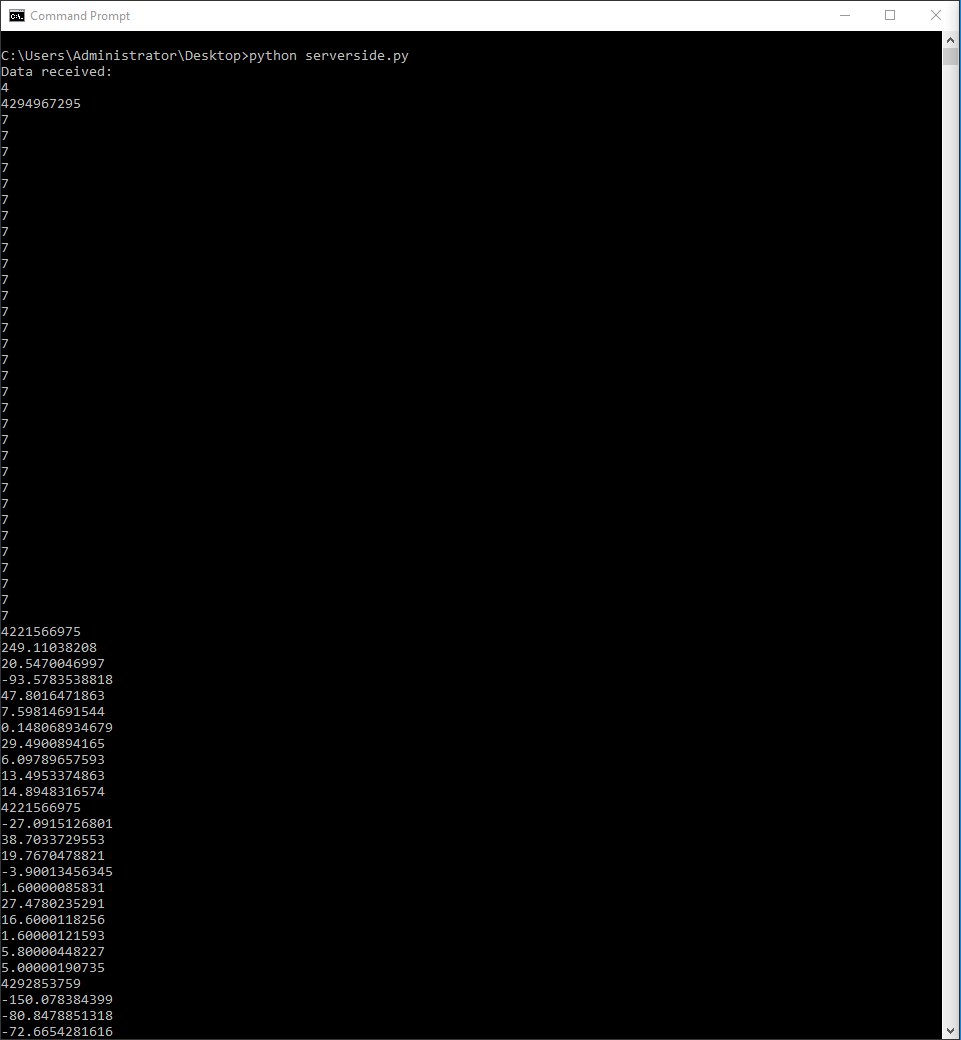
\includegraphics[width=\textwidth]{Figures/unobs_1.png}
\caption{Removing measurements of flows at lines 6-11 and 10-11 and injections at 6,10,11. Part 1}
\label{fig:unobs1}
\end{figure}
\begin{figure}
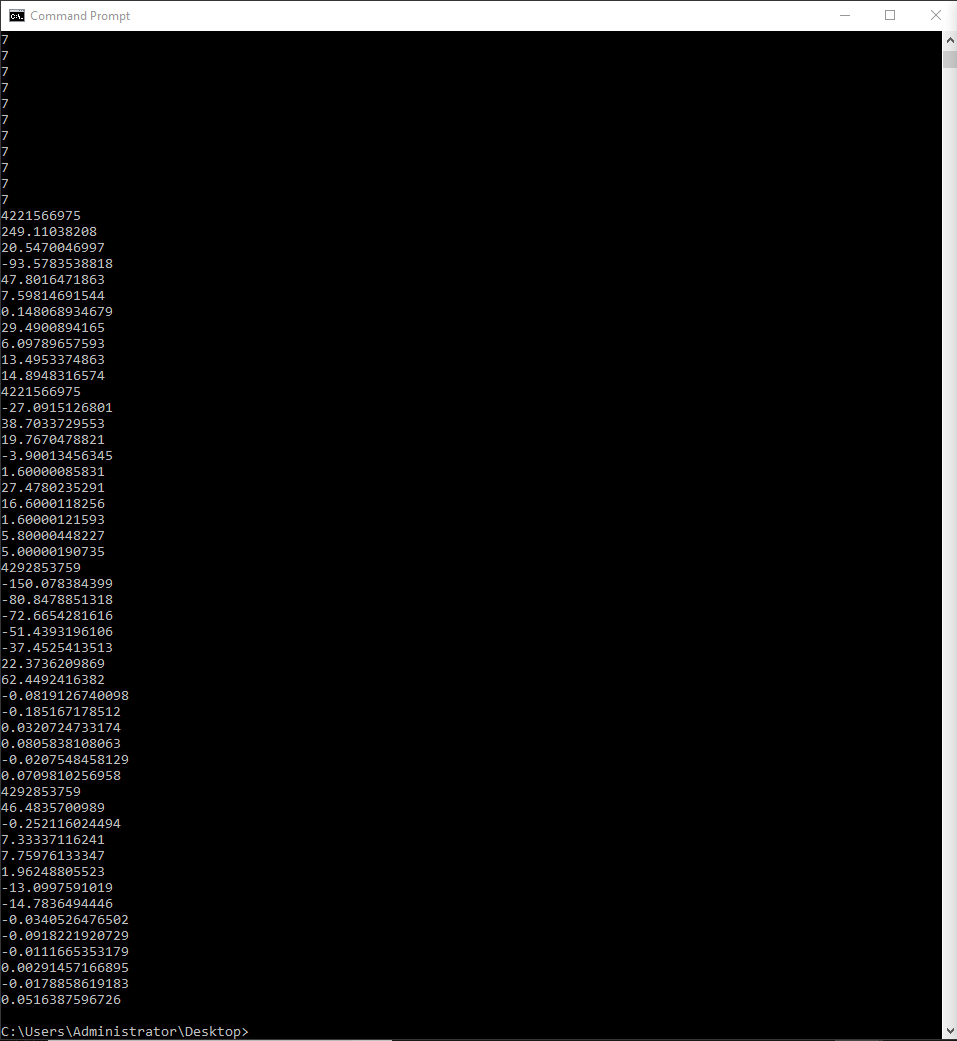
\includegraphics[width=\textwidth]{Figures/unobs_2.png}
\caption{Removing measurements of flows at lines 6-11 and 10-11 and injections at 6,10,11. Part 2}
\label{fig:unobs1}
\end{figure}
\begin{figure}
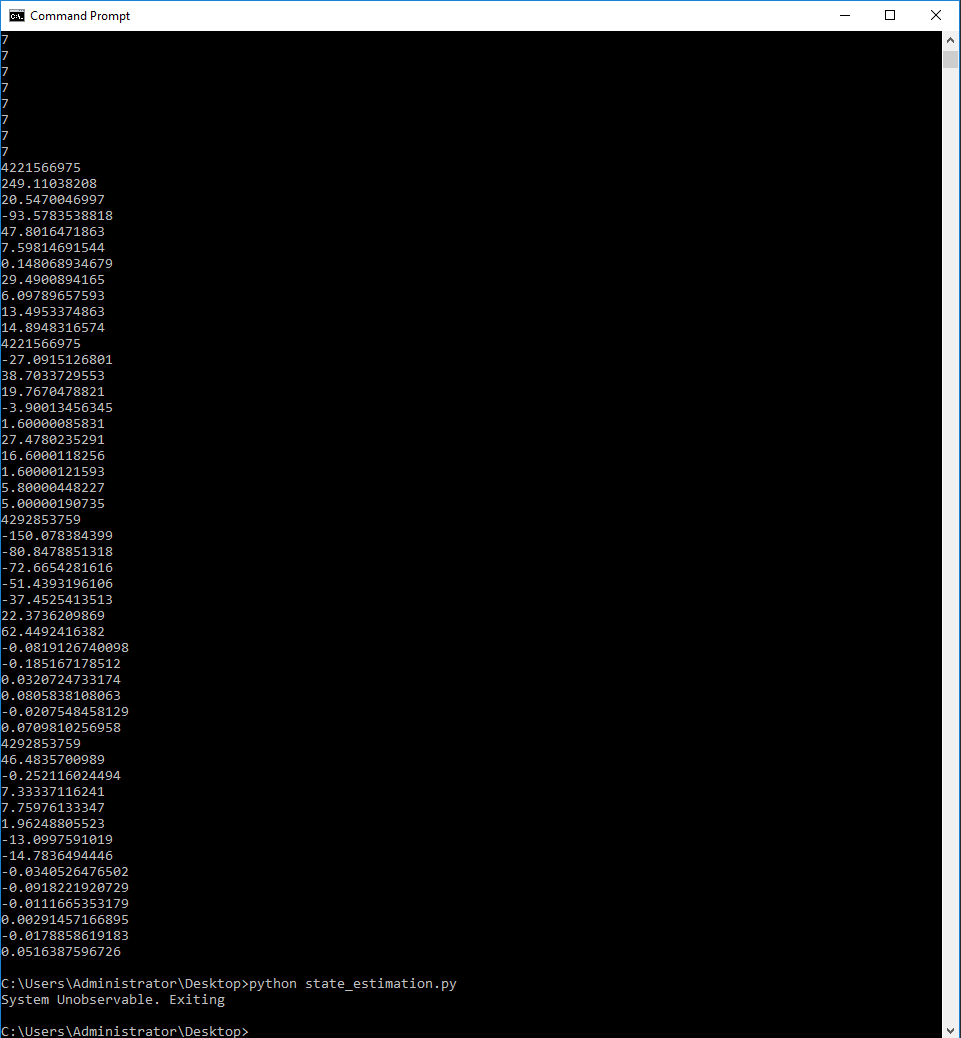
\includegraphics[width=\textwidth]{Figures/non_obs.png}
\caption{Running state estimation with less than neccessary measurements}
\label{fig:unobs1}
\end{figure}
